%-----------------------------------------------------------------------
% Beginning of mcom-l-template.tex
%-----------------------------------------------------------------------
%
%     This is a topmatter template file for MCOM for use with AMS-LaTeX.
%
%     Templates for various common text, math and figure elements are
%     given following the \end{document} line.
%
%%%%%%%%%%%%%%%%%%%%%%%%%%%%%%%%%%%%%%%%%%%%%%%%%%%%%%%%%%%%%%%%%%%%%%%%

%     Remove any commented or uncommented macros you do not use.

\documentclass{mcom-l}

%     If you need symbols beyond the basic set, uncomment this command.
%\usepackage{amssymb}

%     If your article includes graphics, uncomment this command.
\usepackage{graphicx}

%     If the article includes commutative diagrams, ...
%\usepackage[cmtip,all]{xy}


%     Update the information and uncomment if AMS is not the copyright
%     holder.
%\copyrightinfo{2009}{American Mathematical Society}

\newtheorem{theorem}{Theorem}[section]
\newtheorem{lemma}[theorem]{Lemma}

\theoremstyle{definition}
\newtheorem{definition}[theorem]{Definition}
\newtheorem{example}[theorem]{Example}
\newtheorem{xca}[theorem]{Exercise}

\theoremstyle{remark}
\newtheorem{remark}[theorem]{Remark}

\numberwithin{equation}{section}

\begin{document}

% \title[short text for running head]{full title}
\title{}

%    Only \author and \address are required; other information is
%    optional.  Remove any unused author tags.

%    author one information
% \author[short version for running head]{name for top of paper}
\author{}
\address{}
\curraddr{}
\email{}
\thanks{}

%    author two information
\author{}
\address{}
\curraddr{}
\email{}
\thanks{}

%    \subjclass is required.
\subjclass[2010]{Primary }

\date{}

\dedicatory{}

%    Abstract is required.
\begin{abstract}
The paper deals with the values of Hardy's Z-function at generalized Gram points (phi-points, in author's terminology). This question is quite interesting, and some results in this direction can be proved rigorously (these results are cited in the paper). At the same time, the present state of Riemann zeta function theory does not allow one to prove something about value distribution of Z(t) at discrete sequences of points. For example, we are not able 
to prove the analogue of famous Selberg's theorem for the sequence of Gram points. Moreover, possibly these analogues should differ significantly from continuous case. That's why the numerical data have some interest...

\end{abstract}

\maketitle

%    Text of article.

%    Bibliographies can be prepared with BibTeX using amsplain,
%    amsalpha, or (for "historical" overviews) natbib style.
\bibliographystyle{amsplain}
%    Insert the bibliography data here.


%%%%%%%%%%%%%%%%%%%%%%%%%%%%%%%%%%%%%%%%%%%%%%%%%%%%%%%%%%%%%%%%%%%%%%%%

%    Templates for common elements of a journal article; for additional
%    information, see the file Author_Handbook_Journals.pdf, included
%    in the MCOM author package, and the amsthm user's guide, linked
%    from http://www.ams.org/tex/amslatex.html .

%    Section headings
\section{sec1}
a more precise definition for the function $p_{phi}(y)$ is provided.  In particular, note that $|Zeta(1/2+it)|$
 does not possess a limiting distribution (see Laurincikas '' Limit Theorems for the Riemann Zeta-Function" Chapter 3) . 

\subsection{subsec1.1}

%    Ordinary theorem and proof
\begin{theorem}[Optional addition to theorem head]
% text of theorem
\end{theorem}

\begin{proof}[Optional replacement proof heading]
% text of proof
\end{proof}

%    Figure insertion; default placement is top; if the figure occupies
%    more than 75% of a page, the [p] option should be specified.
\begin{figure}
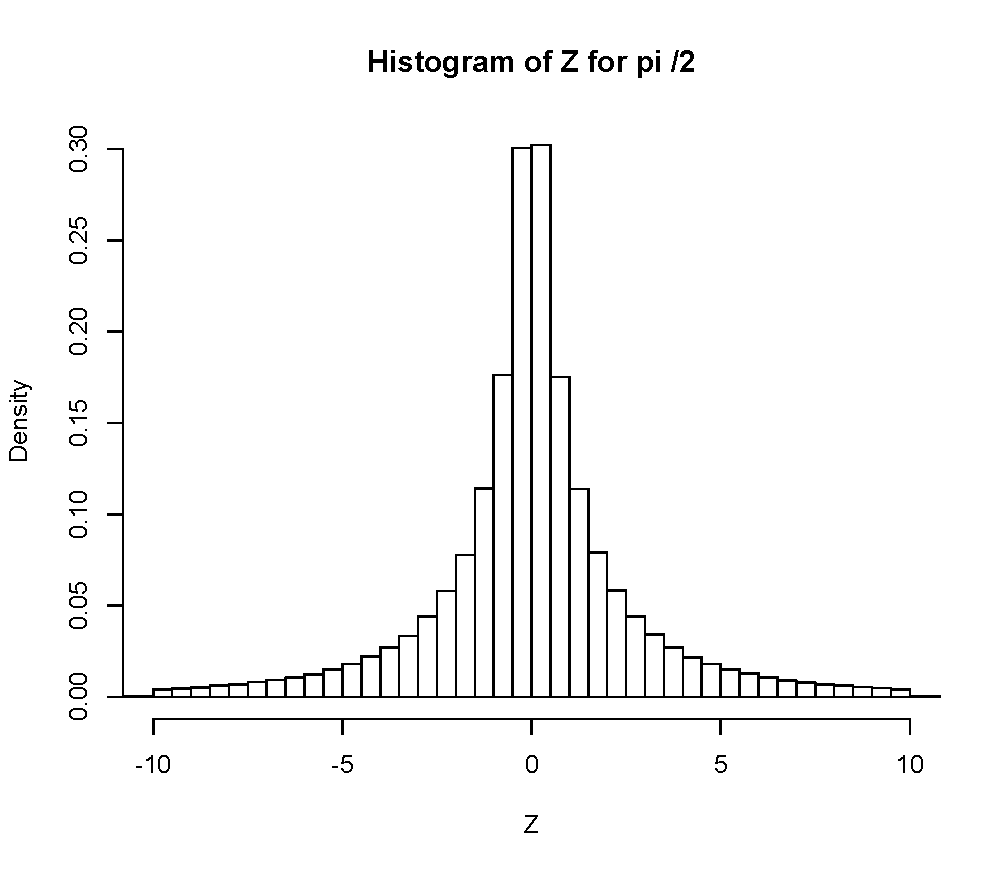
\includegraphics{pi2plot.pdf}
\caption{text of caption}
\label{}
\end{figure}

%    Mathematical displays; for additional information, see the amsmath
%    user's guide, linked from http://www.ams.org/tex/amslatex.html .

% Numbered equation
\begin{equation}
\end{equation}

% Unnumbered equation
\begin{equation*}
\end{equation*}

% Aligned equations
\begin{align}
  & xx \\
  & zz
\end{align}

\end{document}


%-----------------------------------------------------------------------
% End of mcom-l-template.tex
%-----------------------------------------------------------------------
